\subsection{Architecture for classifying single label images}
Figure \ref{singlelabel} shows the Convolutional Neural Network that classifies single label images.In 
the each layer of Convolutional Neural Network from the Figure \ref{singlelabel}, the input image is converted by Spatial Convolution(number of input channels \(\rightarrow\) number of output channels, kernel height x kernel width, step height, step width, padding height, padding width). Then Spatial Batch Normalization is applied. After that Spatial Max Pooling(filter height, filter width, step height, step width) is used to downsample the images. Dropout is used to reduce overfitting. Rectifier Linear Unit is used for activation function. Also Linear Transformation(number of input channels \(\rightarrow\) number of output channels) is used to reduce the number of channels by applying linear transformation.

\begin{figure}[!htb]
  \centering
  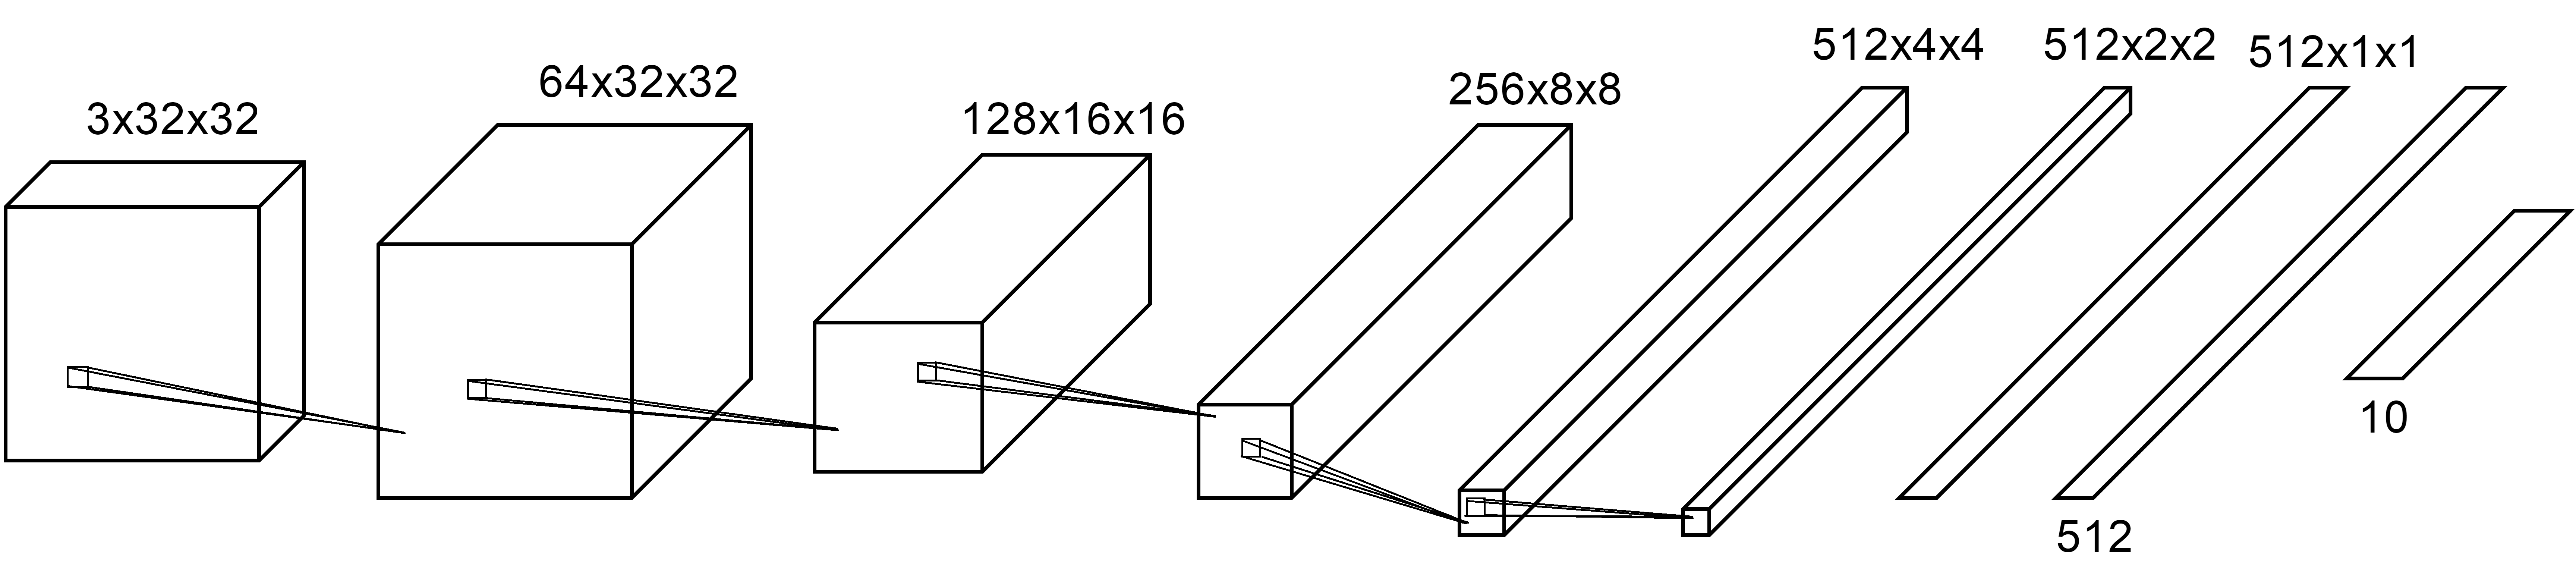
\includegraphics[width=.5\textwidth]{images/singlelabel.png}
  \caption{Convolutional Neural Network for Classifying Single Label Images(Cropped Down)}
   \vspace{-.5cm} \label{singlelabel}
\end{figure} 


 \paragraph{Spatial Convolution}
  
  Applies a 2D convolution over an input image composed of several input planes. For an example, Spatial Convolution(3 \(\rightarrow\) 64, 3x3, 1,1, 1,1) means that number of input channel is 3, and the number of output channel is 64. The kernel size is 3x3 and as there are 64 output channels, there will be 64 kernels, each having dimension 3x3. The step of the convolution is 1 step for height and width. The padding is 1 for height and width. Let's visualize this. In the figure \ref{spatialconv} the input neurons are the ones representing each pixel of an image, the kernel size or the filter size is 5x5. This filter would iterate over every single pixel and for each pixel look at the 5x5 neighborhood and produce corresponding images. As the number of output channel is 64, this will be done 64 times.
  
  \begin{figure}[h!]
  \centering
  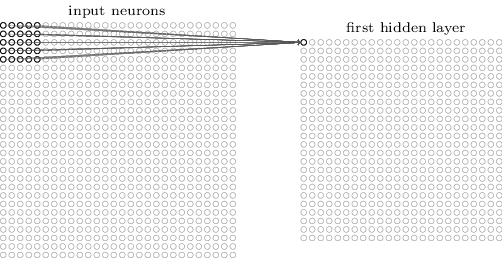
\includegraphics[width=.4\textwidth]{images/spatialconv.png}
  \caption{Spatial Convolution with Kernel Size 5x5} \label{spatialconv}
  \vspace{-.5cm}
\end{figure}

\paragraph{Spatial Batch Normalization}

Implements Batch Normalization as described in the paper FILL. The operation implemented is:

 $$y=\frac{x - mean(x)}{standard \textendash deviation(x)} * gamma + beta$$
 
 where the mean and standard-deviation are calculated per feature-map over the mini-batches and pixels and where gamma and beta are learnable parameter vectors of size N (where N = number of feature maps).
 
 
 \paragraph{ReLU}
 It is the activation function defined as: $$f(x) = max(0,x)$$.
 
 
 \paragraph{Spatial Max Pooling:}
 Applies 2D max-pooling operation. For example, Spatial Max Pooling(2,2,2,2) means that the max pooling will be done with filter 2x2 with step 2 in height and step 2 in width direction. Max pooling means that we will select the maximum value from 2x2 filter or the input area.
 
 
 \paragraph{Dropout}
 Dropout is used to prevent the neural network from overfitting. Dropout is implemented by only keeping a neuron active with some probability p (a hyperparameter), or setting it to zero otherwise. The input neuron is scaled by $1/p$ if it is not deactivated.
 
 \paragraph{Linear}
 Applies a linear transformation to the incoming data ($y = mx + c$). For example, Linear(512 \(\rightarrow\) 10) means that there are 512 input channels and these 512 channels are converted to 10 channels. So, the weight matrix will be 10x512. 
 
 
 \paragraph{Loss Function}
 Cross-entropy loss function has been used which has the form:
 
 
$$ L_{i} = -\log{(\frac{e^{f_y}}{\sum_j{e^{f_j}}})}$$

\paragraph{Normalization on CIFAR-10}

Normalization is required so that all the inputs are at a comparable range. This can be done to force the input values to a certain range. The images were converted from RGB channel to YUV channel. Then U and V channels were normalized globally with mean and standard deviation. The Y channel was normalized locally.

\subsection{Image Segmentation}
\subsubsection{Measuring the objectness of image windows}
B. Alexe et al. \cite{1} presented a generic objectness measure, quantifying how likely it is for an image window to contain an object of any
class. They explicitly trained it to distinguish objects with a well-defined boundary in space, such as cows and telephones, from amorphous
background elements, such as grass and road. The measure combines in a Bayesian framework several image cues measuring characteristics of objects, such as appearing
from their surroundings and having a closed boundary. These include an
innovative cue to measure the closed boundary characteristic. Finally, they presented two applications of objectness. In the first, they sample a small number windows according to their
objectness probability and gave an algorithm to employ them as location priors for modern class-specific object detectors. As they showed 
\begin{figure}[!htb]
    \centering
  \subfloat[a]{%
       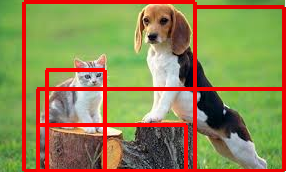
\includegraphics[width=0.4\linewidth]{images/obj1}}
    \label{obj1}
  \subfloat[b]{%
        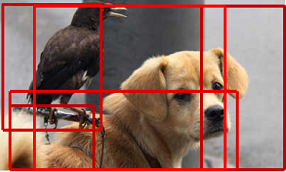
\includegraphics[width=0.4\linewidth]{images/obj2}}
    \label{obj2}
  \caption{Segmented Images}
        \vspace{-.5cm}
  \label{objectnessfig} 
\end{figure}
experimentally, this greatly reduces the number of windows evaluated by the expensive class-specific model. In the second application,
they used objectness as a complementary score in addition to the class-specific model, which leads to fewer false positives. As shown in
several recent papers, objectness can act as a valuable focus of attention mechanism in many other applications operating on image
windows, including weakly supervised learning of object categories, unsupervised pixelwise segmentation, and object tracking in video.
Computing objectness is very efficient and takes only about 4 sec. per image. This technique finds out some image windows like Figure \ref{objectnessfig}.\\
\begin{algorithm}
\SetAlgoLined
\centering
\begin{description}\itemsep0pt \parskip0pt \parsep0pt \vspace{.1cm}
  
  \item[Input:] \(F, D, c\) 
  \item[Ouput:] \(Det\)
  \item[Step 1:] \( \l = \left \{ w_{1},...,w_{F} \right \}, w_{i}\rightarrow D, \forall_{i} \)
  \item[Step 2:] \( \l_{s} = \left \{ \left ( w_{1},sw_{1} \right ),...,\left ( w_{F},sw_{F} \right )  \right \}, sw_{i}= c\left ( w_{i} \right ), \forall_{i} \) 
  \item[Step 3:] \( \rho _{s} = NMS\left ( \l_{s} \right )=\left \{ \left ( w_{n1},sw_{n1} \right ),...,\left ( w_{np},sw_{np} \right )  \right \}\)
  \item[Step 4:] \(\L=\left \{ w_{n1}^{lm},..., w_{np}^{lm} \right \}, w_{nj}^{lm} = max \left ( s_{w} \right )\)
  \item[Step 5:] \(Det = NMS\left ( \L \right )\)
\end{description}
\caption{Using objectness for class-specific detectors.}
\end{algorithm}
The general scheme for using their objectness measure as
a location prior for object detectors is algorithm 1. The
algorithm inputs the class-specific confidence function \(c\) which
the detector employs to score a window.
They build an initial set \(\l\) of \(F = 1000\) windows multinomially sampled from the distribution \(D\) of windows scored by
their objectness measure (Multi-scale Saliency)\(MS\) +(Color Contrast)\(CC\) + (Superpixels Straddling)\(SS\) (step 1). They use \(c\) to
score each window in \(\l\) (step 2). They then run the non-maxima
suppression. This results in a set \(\rho_{s}\) of promising
windows (step 3). For every window \(w_{p} \epsilon \rho_{s}\), they iteratively
move to the local maximum of \(c\) in its neighborhood \(V_{w
p}\),
resulting in window \(w_{p}^{lm}\) (step 4). Finally, they run \(NMS\) on the
local maxima windows \(\L\) and obtain detections \(Det\) (step 5).
In order to use this algorithm one has to specify a window
scoring function \(c\), which is specific to a particular detector
and object class, and a window neighborhood.

\subsubsection{Selective Search for Object Recognition}

J.R.R. Uijlings et al. \cite{2} took a hierarchical grouping algorithm to form the basis of their
selective search. Bottom-up grouping is a popular approach to segmentation, hence they adapted it for selective search. Because
the process of grouping itself is hierarchical, they can naturally generate locations at all scales by continuing the grouping process until
the whole image becomes a single region. This satisfies the condition of capturing all scales.
As regions can yield richer information than pixels, they wanted to
use region-based features whenever possible. To get a set of small
starting regions which ideally do not span multiple objects, they used the fast method of Felzenszwalb and Huttenlocher \cite{7}, which
found well-suited for such purpose.
Their grouping procedure now works as follows. They first used \cite{7}
to create initial regions. Then they used a greedy algorithm to iteratively group regions together: First the similarities between all
neighbouring regions are calculated. The two most similar regions
are grouped together, and new similarities are calculated between
the resulting region and its neighbours. The process of grouping
the most similar regions is repeated until the whole image becomes
a single region.


\subsection{Architecture For Classifying Multi-Label Images}

Our Final architecture for detecting multi-label images consists of (1) image segmentation and (2) convolutional neural network for detecting segmented images. The image segmentation techniques, objectness measures and selective search and the architecture for single label image detection has been described before. In the Figure \ref{finalarch} there is an overview of the architecture.
\begin{figure}[!htb]
  \centering
  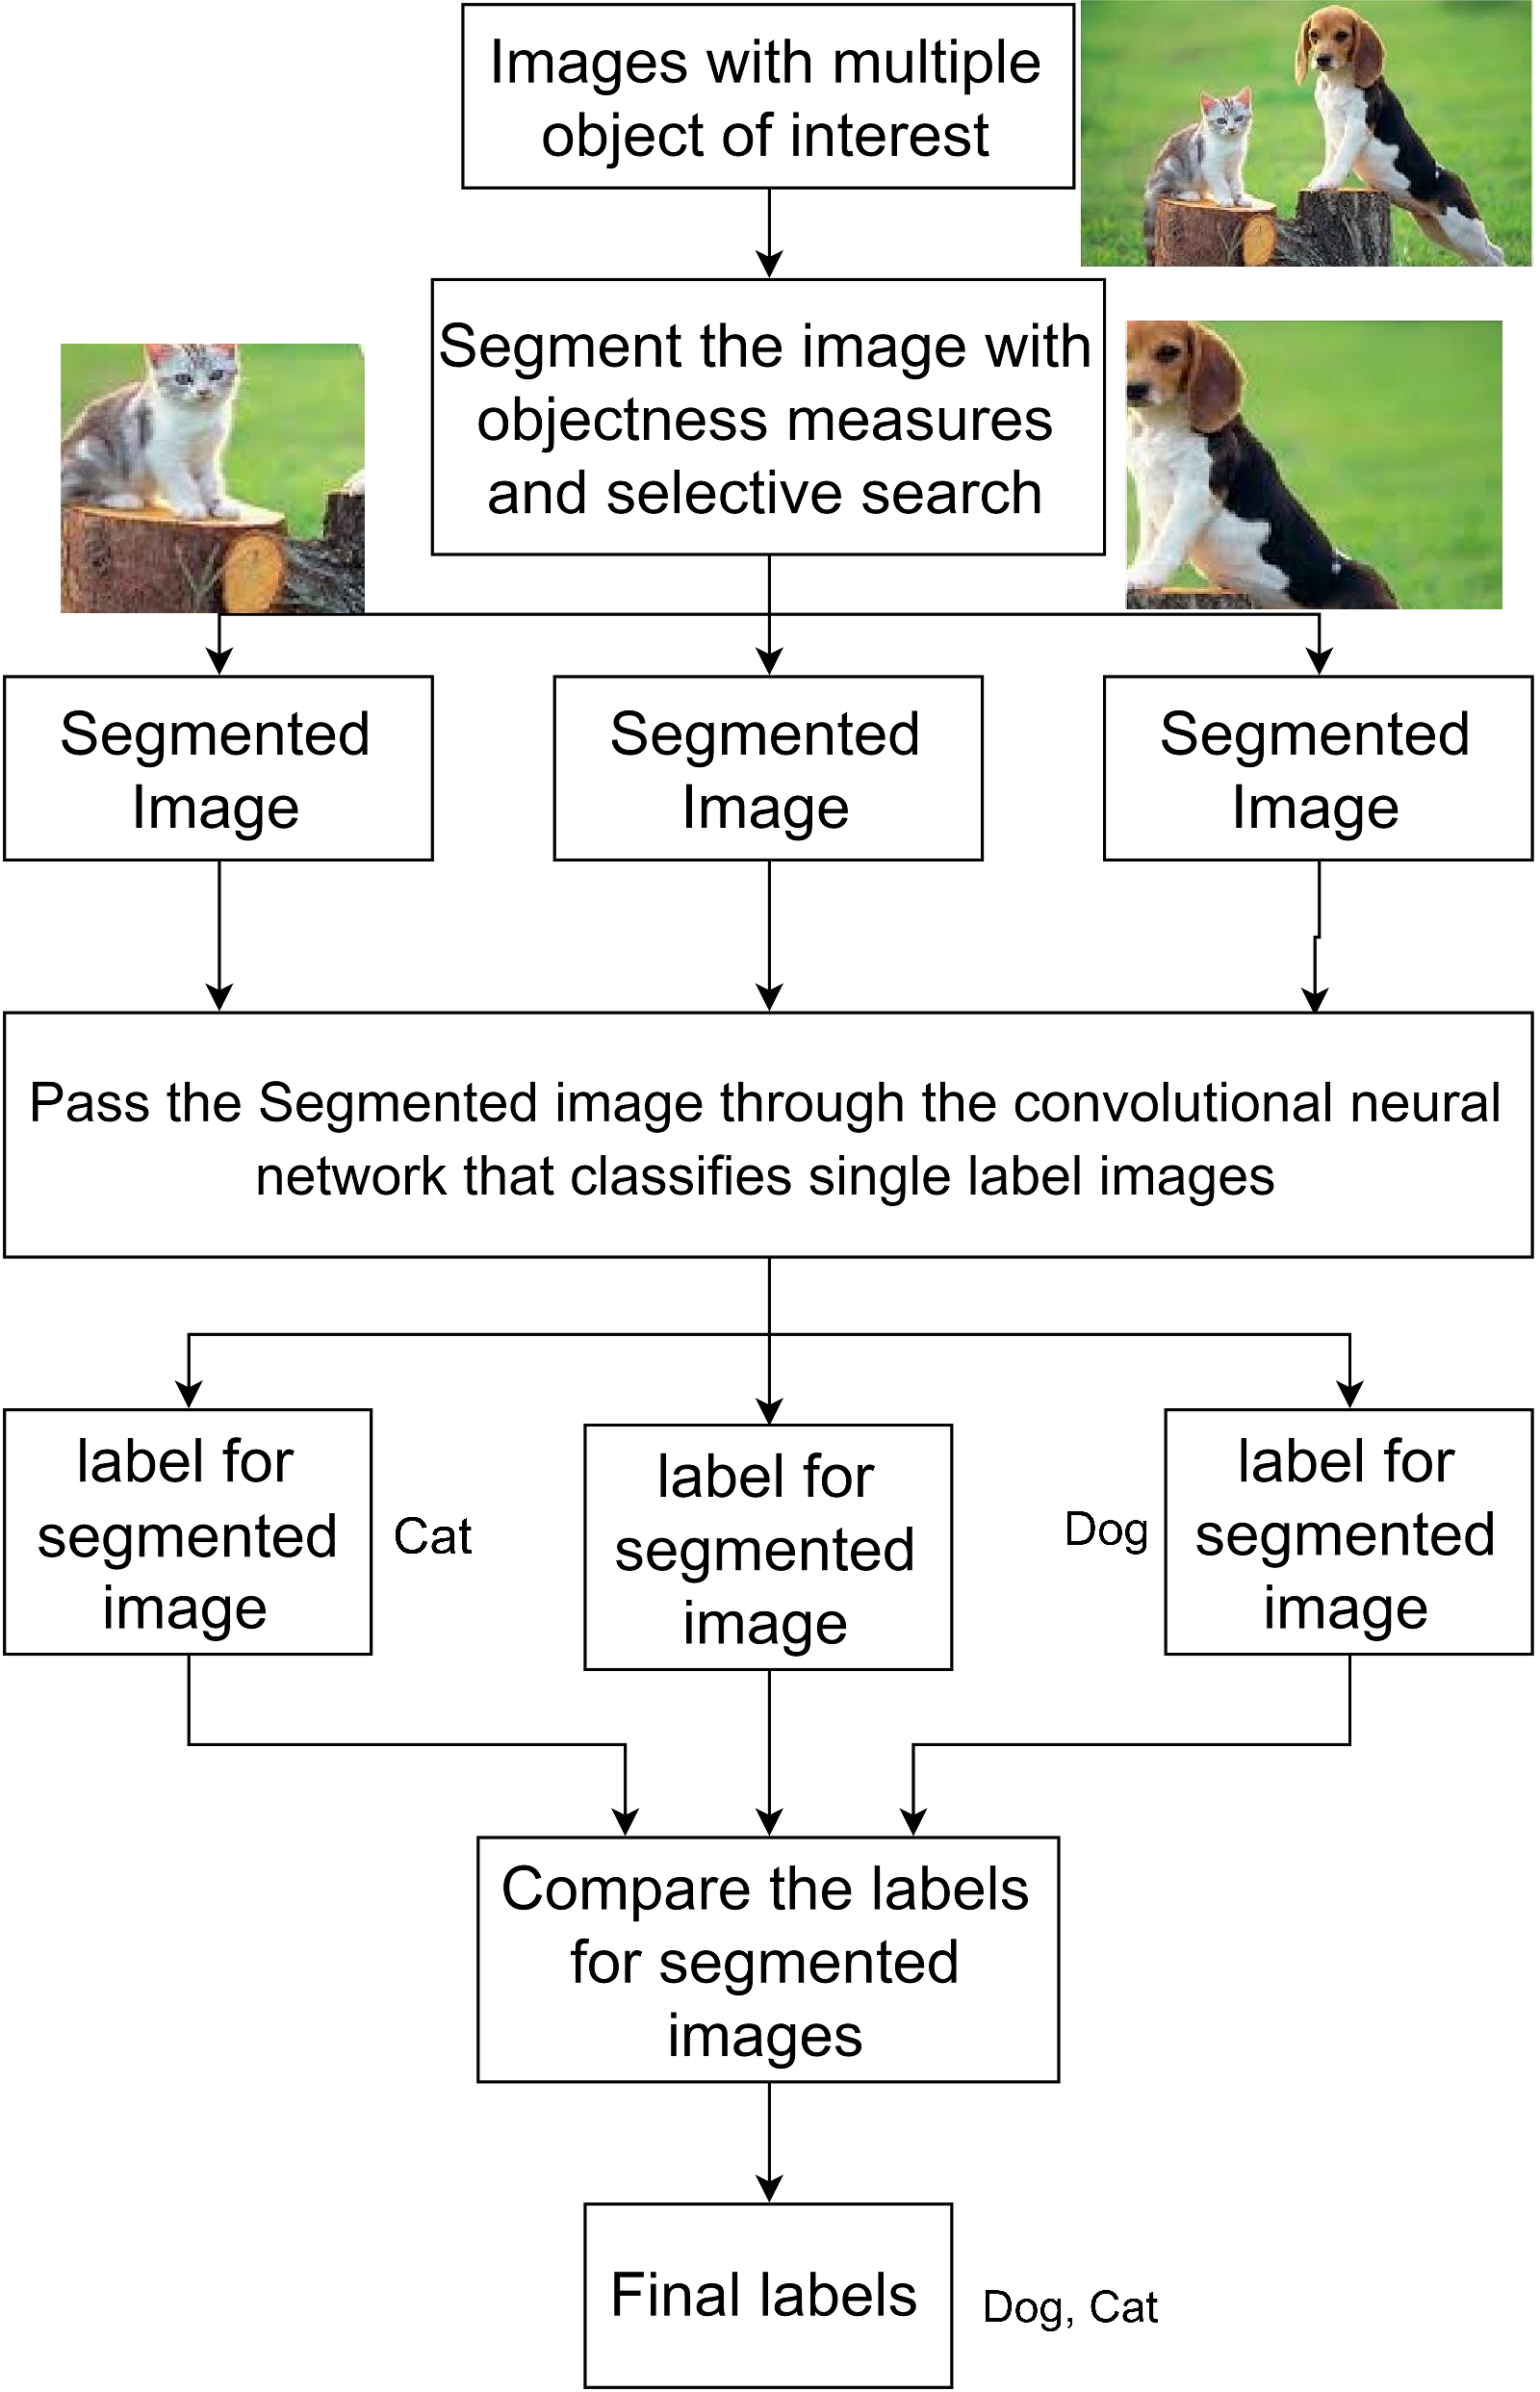
\includegraphics[width=0.4\textwidth]{images/finalarch.png}
  \caption{Architecture of Convolutional Neural Network}\label{finalarch}
\end{figure}
At first we split the image with objectness measures and selective search. Then we get multiple split images. Note that there will be many split images. In the figure only a few are shown. Then we pass the split images through the convolutional neural network that classifies the label associated with that image. As there are many split images, there may be some labels that will be wrongly classified. We inspect these labels and their associative scores and finally conclude which of the labels are likely to be associated with the images. We performed several techniques for inspecting the images. These are discussed in the experimental result section.
